\begin{frame}{Gradient Boosting: Khái niệm Cơ bản}
    \begin{columns}[T]
        \begin{column}{0.59\textwidth}
            Gradient Boosting xây dựng chuỗi bộ học yếu theo kiểu tuần tự:
            \begin{itemize}
                \item Mô hình sau học từ lỗi của mô hình trước
                \item Tối ưu dần phần dư (residuals)
                \item Dự đoán cuối là tổng có trọng số
            \end{itemize}
        \end{column}

        \begin{column}{0.4\textwidth}
            \centering
            % \fbox{\parbox[c][2.9cm][c]{0.9\linewidth}{\centering Ch\`en h\`inh minh h\d{o}a chu\~oi boosting v\`ao \^o n\`ay}}
            % Sau khi co anh, co the thay bang:
            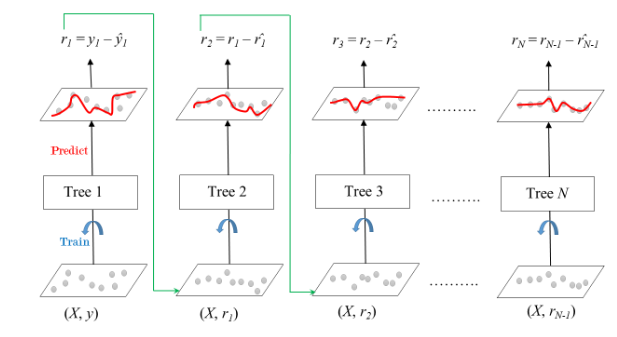
\includegraphics[width=0.95\linewidth]{img/gradientboosting.png}
        \end{column}
    \end{columns}

                \begin{block}{Ý tưởng chính}
                \begin{enumerate}
                    \item Huấn luyện mô hình đầu tiên
                    \item Tính sai số còn lại
                    \item Huấn luyện mô hình mới để sửa sai số đó
                \end{enumerate}
            \end{block}
\end{frame}

\begin{frame}{Gradient Boosting: Quy trình và Tuning}
                \begin{itemize}
                    \item Khởi tạo mô hình yếu ban đầu
                    \item Với mỗi vòng lặp: học trên residuals
                    \item Cập nhật: $f_t(x) = f_{t-1}(x) + lr \cdot h_t(x)$
                    \item Lặp đến $n\_estimators$
                \end{itemize}

            \begin{block}{Regularization chính}
                \begin{itemize}
                    \item \textbf{learning\_rate}: nhỏ hơn $\Rightarrow$ học chậm, ổn định hơn
                    \item \textbf{subsample} $< 1$: Stochastic GB, giảm overfitting
                \end{itemize}
            \end{block}
\end{frame}

\begin{frame}[shrink=10]{Gradient Boosting: Đánh giá}
    \begin{columns}[T]
        \begin{column}{0.48\textwidth}
            \textbf{Ưu điểm:}
            \begin{itemize}
                \item Độ chính xác cao trên dữ liệu có pattern phức tạp
                \item Tập trung sửa lỗi từng bước
                \item Linh hoạt với nhiều hàm mất mát
            \end{itemize}
        \end{column}
        \begin{column}{0.48\textwidth}
            \textbf{Nhược điểm:}
            \begin{itemize}
                \item Dễ overfitting nếu tuning chưa tốt
                \item Huấn luyện chậm hơn Bagging do tính tuần tự
                \item Nhạy với hyperparameters
            \end{itemize}
        \end{column}
    \end{columns}

    \begin{alertblock}{Kết quả mẫu (Breast Cancer)}
        Cấu hình: $n\_estimators=100$, $learning\_rate=0.1$, $subsample=0.5$:
        \begin{itemize}
            \item \textbf{bAcc}: 0.94
            \item \textbf{AUC}: 0.98
            \item So với SVM: thấp hơn nhẹ; so với RF: nhỉnh hơn bAcc
        \end{itemize}
    \end{alertblock}

    \hfill{\scriptsize \cite{duchesnay2021statsml}}
\end{frame}
